\chapter{Methodology}
\label{chapterlabel3}

\section{Research Design and Analytical Framework}

The study adopts a sequential quantitative framework in which night-time public transport usage types are first identified from transport data and subsequently interpreted in relation to external area-level contexts.

First, temporal profiles were constructed separately for Rail stations and bus-served LSOAs. Rail profiles were based on station entries and exits, while Bus profiles were based on area-level boardings and estimated alightings. The two modes were analysed separately because their source data, temporal resolutions, spatial units and feature constructions differ.

Second, Gaussian Mixture Models were used to identify night-time usage patterns. The resulting cluster solutions were evaluated using fitted-model evidence, stability diagnostics, separation measures and the substantive interpretability of their temporal profiles.

After cluster assignment, activity volume, directional balance, late-night persistence and other behavioural descriptors were used to characterise the fixed clusters; these descriptors were not used to redefine cluster membership.

Third, the fixed cluster solutions were examined in relation to the London Night Workers Classification and 20 continuous urban background indicators. These contextual variables provided an external interpretive layer for assessing whether different observed-use types occurred within different night-work and socio-spatial environments.

\begin{figure}[H]
\centering
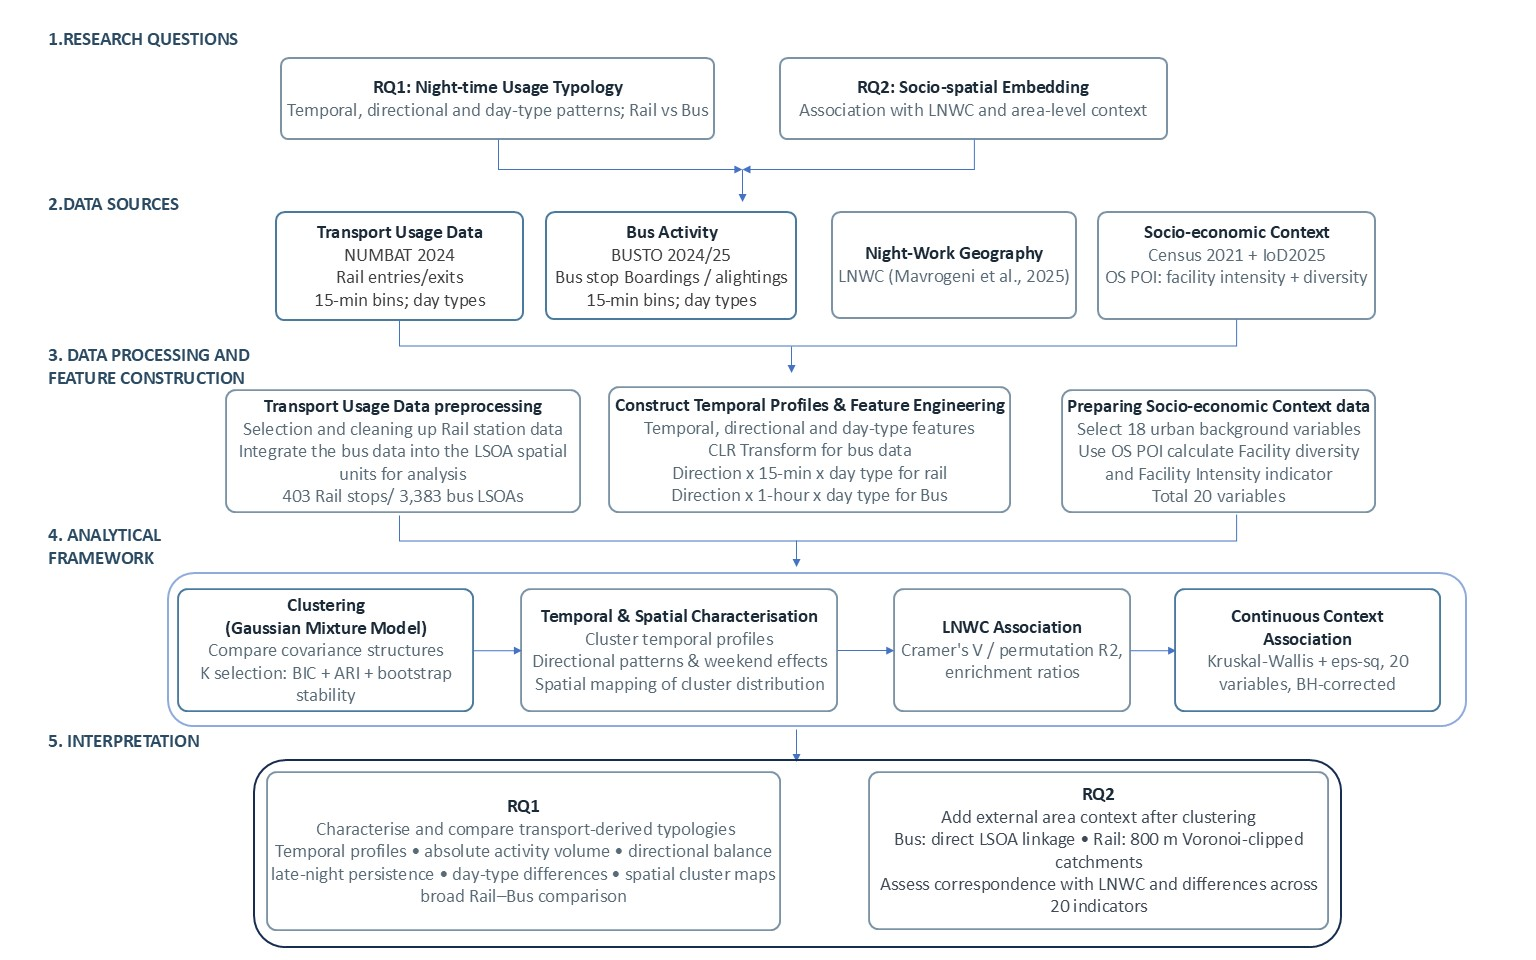
\includegraphics[width=\textwidth]{figures/v5_ch3_fig1.jpg}
\caption[Research framework]{Research framework and structure}
\end{figure}

\section{Data and Preparation}

\subsection{Rail Passenger Activity: NUMBAT 2024}

Rail passenger activity was derived from Transport for London's NUMBAT 2024 dataset \citep{TfL2024NUMBAT}. NUMBAT reports station entries and exits at 15-minute intervals for five representative day types within a typical operational week in autumn 2024.

Each operational day runs from 05:00 to 04:59 on the following calendar day. The dataset covers the London Underground, Docklands Light Railway, London Overground and Elizabeth line.

NUMBAT represents typical-day activity rather than continuous observations for every operating date. So, the data capture representative temporal patterns but do not describe day-to-day disruption or seasonal variation.

The raw data contained 471 station codes, some of which represented separate entry/exit systems for the same interchange rather than distinct locations. Twenty-nine such codes were merged into 14 co-located station units by aggregating activity across day type, direction and time interval, resulting in 456 physical stations. These were matched to NaPTAN \emph{(National Public Transport Access Nodes)} records; 16 without a Greater London match and 37 tram-only units with no recorded activity were excluded. The final Rail dataset comprised 403 spatially referenced stations.

A fixed night-time window of 18:00--05:00 was applied to all five-day types. This produced 44 quarter-hour observations per day type and direction. Intervals following the end of service were retained as zero values rather than removed, maintaining a common feature length across day types while preserving the limited post-01:00 activity recorded on non-Night-Tube days by services such as the Elizabeth line and London Overground.

Each Rail station was therefore represented by 440 normalised features: 220 quarter-hour shares for entries and 220 for exits. Entry and exit profiles were retained separately for subsequent feature construction and clustering.

\subsection{Bus Passenger Activity: BUSTO 2024/25}

Bus passenger activity was obtained from TfL's BUSTO 2024/25 Total Demand dataset \citep{TfL2025BUSTO}. BUSTO reports passenger activity by route, direction, StopPoint and 15-minute interval for three representative day types: Weekday, Saturday and Sunday. Boarding values are derived from recorded passenger activity, whereas alighting values are estimated by TfL. The data should also be interpreted as representative measures of bus activity.

The release comprised 12 route-group and day-type files covering numbered and letter-prefix bus routes. Unlike NUMBAT, BUSTO does not distinguish Friday from other weekdays, so Friday-night activity could not be analysed separately.

Because individual StopPoints often recorded low night-time flows and unstable temporal profiles, Bus activity was aggregated to 2021 LSOAs to provide a more stable spatial unit for temporal profiling and clustering. Before spatial assignment, StopPoints were first grouped using the official NaPTAN StopArea hierarchy, while those without a parent StopArea were kept as individual units. Passenger activity was then summed within each StopArea or individual StopPoint before assignment to LSOAs. This reduced 19,589 StopPoints to 12,007 spatial units. Of these, 10,879 were located within Greater London and contributed positive night-time activity to 3,797 LSOAs.

The records were then reconstructed into a continuous analytical night from 18:00 to 05:00. Because the source files are organised by calendar day, evening and post-midnight observations were recombined to represent each night: weekday evenings were paired with weekday post-midnight records, Saturday evenings with Sunday post-midnight records, and Sunday evenings with weekday post-midnight records. Following TfL's recommendation \citep{TfL2025BUSTO}, the original 15-minute observations were subsequently aggregated to 11 hourly intervals per day type and direction, reducing the influence of very small quarter-hour values on temporal profiling.

A minimum-activity threshold was applied because very low-volume LSOAs produced sparse and unstable directional profiles. Following the low-activity screening principle used by \citet{MarinasCollado2022}, an analogous threshold was adapted to the present data structure. Each LSOA was required to record at least 33 passenger activities (11 hourly intervals $\times$ 3 day types) separately in both the boarding and alighting directions, equivalent to an average of at least one activity per hourly component in each direction. This retained 3,383 of the 3,797 LSOAs with positive night-time activity.

Each retained LSOA was represented by 66 temporal observations: 11 hourly intervals $\times$ 3 day types $\times$ 2 directions. The final Bus analytical dataset comprised 3,383 LSOAs with hourly boarding and estimated-alighting profiles for subsequent feature construction and clustering.

\subsection{Urban Night Contextual Data and Preparation}

To interpret observed transport-use patterns in relation to their surrounding urban context, the study used the London Night Workers Classification (LNWC) alongside area-level socio-economic, demographic and functional indicators.

\subsubsection{London Night Workers Classification}

The London Night Workers Classification (LNWC) was used as an independent area-context layer for interpreting the transport clusters. Developed by Mavrogeni, Cheshire, Iliev and van Dijk as part of the Data After Dark programme \citep{Mavrogeni2025}, the LNWC combines mobile-phone footfall data with business-location data from the Directory of London Businesses. Businesses are classified using SIC codes to identify sectors associated with night-time work, and London LSOAs are grouped into seven area types representing different night-working contexts. Because the LNWC was constructed independently of the smart-card transport profiles analysed here, it provides an external reference for examining whether different transport-use types occur within different night-work contexts.

\begin{table}[H]
\centering
\small
\resizebox{\textwidth}{!}{%
\begin{tabular}{@{}c p{3.1cm} p{4cm} p{5.2cm}@{}}
\toprule
LNWC & Short name & Night-worker presence & Night-time-economy business presence \\
\midrule
1 & Central night-work hubs & Much higher than average, all time windows, peaking 18:00--21:00 weekdays & Much higher than average across all categories (arts/recreation, hospitality, retail dominant) \\
2 & Inner suburbs, high night business & Higher than average & Above average across most categories \\
3 & Inner suburbs, low night business & Higher than average (comparable to LNWC 2) & Below average; workers concentrated outside the tracked NTE categories (e.g.\ airport operations, building cleaning) \\
4 & Suburban business, average activity & Average & Above average, led by security, hospitality, transport and storage \\
5 & Suburban transport \& health, low activity & Lower than average & Broadly average; transport, storage and health slightly above \\
6 & Low-activity suburban & Lower than average (comparable to LNWC 5) & Below average across all categories \\
7 & Night-worker periphery & Extremely low, especially 03:00--06:00 weekdays & Below average across all categories \\
\bottomrule
\end{tabular}%
}
\caption[LNWC cluster types]{LNWC cluster types (adapted from \citealp{Mavrogeni2025})}
\end{table}

\begin{figure}[H]
\centering
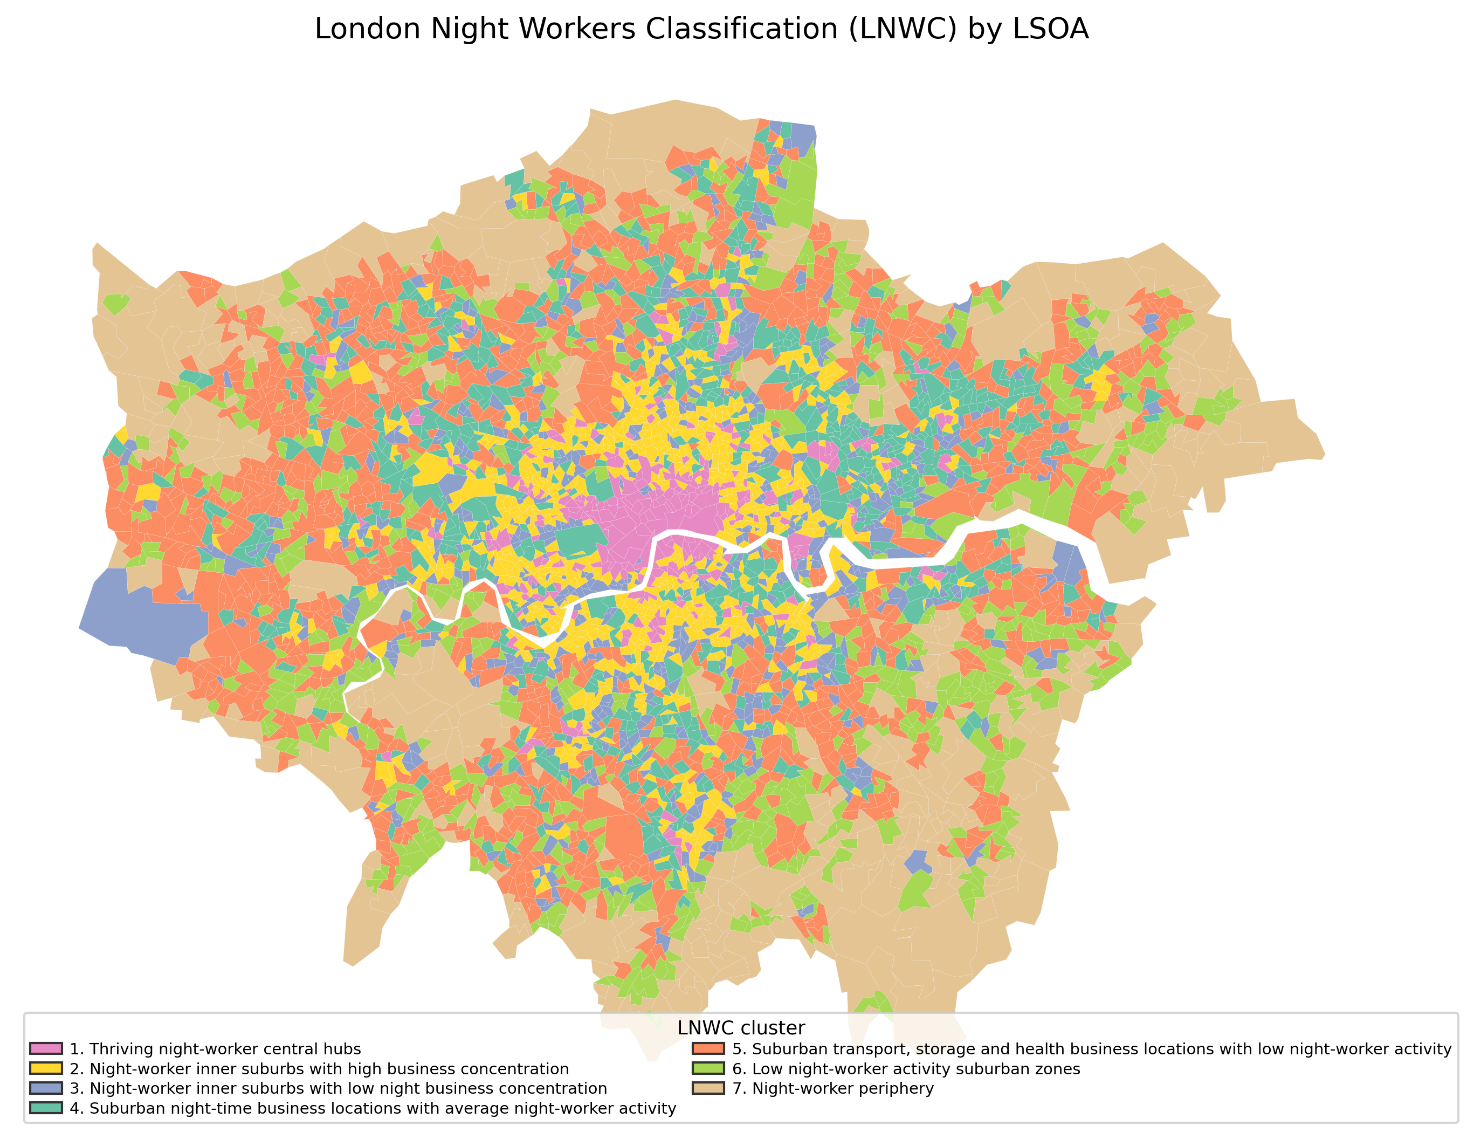
\includegraphics[width=\textwidth]{figures/v5_ch3_lnwcmap.png}
\caption[LNWC spatial distribution]{Spatial distribution of the seven London Night Workers Classification (LNWC) types across Greater London. Colours follow \citet{Mavrogeni2025}.}
\end{figure}

\subsection{Socio-economic, Demographic and Functional Indicators}

The socio-economic and demographic contextual analysis draws on two main sources: the 2021 UK Census provided by the Office for National Statistics (ONS) \citep{ONS2021} and the English Indices of Deprivation 2025 (IoD2025) \citep{MHCLG2025}. The LSOA was retained as the common source geography to ensure spatial consistency across the contextual indicators. Based on the relevant literature, 18 variables were selected to represent different dimensions of local context, including deprivation, housing, car ownership, demographic structure, and residence-based employment in night-time-economy industries. The specific variables are summarised in the following table.

The selection of these variables was informed by previous studies examining socio-economic and demographic characteristics associated with human mobility patterns \citep{Long2015,Cao2019,Zhang2019,SariAslam2021,Yang2023}. Residence-based employment in night-time-economy industries was defined with reference to the SIC-based industry categories used in the LNWC \citep{Mavrogeni2025}.

\small
\begin{longtable}{@{}p{2.8cm} p{3.0cm} p{2.4cm} p{4.6cm}@{}}
\caption[Contextual variables]{Socio-economic and night-time employment variables} \\
\toprule
Domain & Variable & Source & Description \\
\midrule
\endfirsthead
\multicolumn{4}{l}{\small\itshape (Table \thetable\ continued)} \\
\toprule
Domain & Variable & Source & Description \\
\midrule
\endhead
\bottomrule
\multicolumn{4}{r}{\small\itshape (continued on next page)} \\
\endfoot
\bottomrule
\endlastfoot
Area Deprivation & Education Skills and Training score & IoD2025 & LSOA domain deprivation score for education and skills \\
Area Deprivation & Health Deprivation and Disability score & IoD2025 & LSOA domain deprivation score for health and disability \\
Area Deprivation & Deprived in $\geq$1 dimension (\%) & Census 2021, TS011 & Share of households deprived in at least one of four Census deprivation dimensions \\
Housing \& Car Ownership & Social rented (\%) & Census 2021, TS054 & Share of households in social rented tenure \\
Housing \& Car Ownership & Private rented (\%) & Census 2021, TS054 & Share of households in private rented tenure \\
Housing \& Car Ownership & No car or van (\%) & Census 2021, TS045 & Share of households with no car or van available \\
Household \& Demographic Structure & Dependent children (\%) & Census 2021, TS003 & Share of households with dependent children \\
Household \& Demographic Structure & Population density & Census 2021, TS001 & Usual residents per km$^2$ \\
Ethnicity & Asian ethnicity (\%) & Census 2021, TS021 & Share of usual residents identifying as Asian ethnic group \\
Ethnicity & Black ethnicity (\%) & Census 2021, TS021 & Share of usual residents identifying as Black ethnic group \\
Economic Activity & Unemployed (\%) & Census 2021, TS066 & Share of economically active residents aged 16+ who are unemployed \\
Night-time Industry (residence) & Accommodation \& food services (\%) & Census 2021, TS060A & Share of employed residents (16+) working in hospitality-related industries \\
Night-time Industry (residence) & Transport \& storage (\%) & Census 2021, TS060A & Share of employed residents working in transport and storage industries \\
Night-time Industry (residence) & Administrative \& support services (\%) & Census 2021, TS060A & Share of employed residents working in administrative/support-service industries (proxy for security-related occupations) \\
Night-time Industry (residence) & Wholesale \& retail trade (\%) & Census 2021, TS060A & Share of employed residents working in wholesale and retail industries \\
Night-time Industry (residence) & Human health \& social work (\%) & Census 2021, TS060A & Share of employed residents working in health and social-care industries \\
Night-time Industry (residence) & Manufacturing (\%) & Census 2021, TS060A & Share of employed residents working in manufacturing industries \\
Age structure & Aged 20--34 (\%) & Census 2021, TS007b & Share of residents aged 20 to 34 \\
Environment & POI count & Ordnance Survey Points of Interest & Total number of points of interest within the LSOA \\
Environment & POI Diversity (Shannon H) & Ordnance Survey Points of Interest & Shannon diversity index across the nine top-level OS POI groups \\
\end{longtable}

Ordnance Survey Points of Interest (POI; June 2026 release, accessed through EDINA Digimap) \citep{OSPOI2026} were used to characterise the functional environment of each area. Drawing on previous studies, two indicators were derived from the POI data: facility intensity and functional diversity \citep{PeiretGarcia2026}.

Facility intensity was measured as the total number of POIs within each LSOA and was transformed using $\log(1+x)$ to reduce the influence of the strongly right-skewed count distribution. Functional diversity was measured using the Shannon index across the nine top-level OS POI groups:

\begin{equation}
H = -\sum_{g=1}^{G} p_g \ln(p_g),
\end{equation}

where $p_g$ is the proportion of POIs belonging to group $g$. Larger values indicate a more even distribution across facility groups.

Together, the 18 Census and deprivation indicators and the two POI measures produced a set of 20 continuous contextual variables. These were calculated at LSOA level and linked directly to Bus units or aggregated across Rail station catchments using the procedure described in Section 3.3.4.1.

\section{Analytical Methods}

\subsection{Feature Engineering}

Following data preparation, the Rail and Bus temporal profiles were converted into feature spaces suitable for clustering. Feature construction was designed to emphasise differences in the temporal shape of public transport activity rather than differences in absolute passenger volume.

\subsubsection{Direction-specific Normalisation}

Night-time passenger activity is highly uneven across London, with major interchanges and central locations recording substantially greater volumes than most other units. Clustering raw passenger counts might risk grouping locations primarily according to activity scale rather than according to when they are used.

To focus the classification on temporal structure, activity was normalised separately for each unit and direction across the complete analytical period, following approaches used in previous temporal mobility research \citep{Briand2016,ElMahrsi2017,Verma2021}.

For unit $i$, direction $d$ and time component $t$, the normalised share was:

\begin{equation}
p_{i,d,t} = \frac{c_{i,d,t}}{\sum_{t'} c_{i,d,t'}}, \qquad \sum_{t} p_{i,d,t} = 1 \quad \forall\ i,d
\end{equation}

where $c_{i,d,t}$ is the recorded or estimated activity and the denominator is the unit's total activity in direction $d$ across the complete analytical period.

Rail entries and exits were normalised separately, as were Bus boardings and alightings.

Each directional profile entered the clustering feature space independently, limiting the influence of differences in absolute directional volume on cluster assignment.

Absolute passenger activity was retained separately and reintroduced after clustering as a behavioural descriptor.

\subsubsection{Compositional Transformation of Bus Features}

Direction-specific normalisation produces compositional profiles in both modes because the shares within each direction sum to one and cannot vary independently.

An increase in one interval necessarily reduces the shares available to the others, so ordinary Euclidean distances may distort their relative structure \citep{Aitchison1982}. The adopted Bus model addresses this constraint through a CLR transformation of its 33 hourly components. Rail retains the normalised raw-share representation across 220 quarter-hour components per direction as a pragmatic modelling choice; the remaining compositional constraint is recognised as a limitation rather than assumed to be negligible.

To represent relative differences between intervals in an unconstrained coordinate space, the adopted Bus specification applied a centred log-ratio (CLR) transformation separately to the boarding and alighting profiles.

Because the CLR transformation requires strictly positive components, zero values were first replaced using a prior-weighted Bayesian-multiplicative procedure \citep{MartinFernandez2015}.

For LSOA $i$, direction $d$ and concatenated day-type--hour component $t$, the network-wide temporal prior was defined as:

\begin{equation}
\pi_{dt} = \frac{\sum_i c_{idt}}{\sum_i \sum_{t'} c_{idt'}}.
\end{equation}

The zero-adjusted composition was then calculated as:

\begin{equation}
\widetilde{p}_{idt} = \frac{c_{idt} + \alpha \pi_{dt}}{\sum_{t'} c_{idt'} + \alpha}, \qquad \alpha = 1.
\end{equation}

Thus, one notional observation was distributed across the 33 temporal components in proportion to the corresponding network-wide activity shares. This preserved the observed temporal structure of the network rather than replacing every zero with the same arbitrary constant.

The adjusted composition was transformed as:

\begin{equation}
z_{idt} = \ln\!\left( \frac{\widetilde{p}_{idt}}{g(\widetilde{\mathbf{p}}_{id})} \right), \qquad g(\widetilde{\mathbf{p}}_{id}) = \left( \prod_{t=1}^{D} \widetilde{p}_{idt} \right)^{1/D},
\end{equation}

or equivalently,

\begin{equation}
z_{idt} = \ln(\widetilde{p}_{idt}) - \frac{1}{D} \sum_{s=1}^{D} \ln(\widetilde{p}_{ids}).
\end{equation}

The transformed components sum to zero within each direction, and Euclidean distance in CLR coordinates corresponds to Aitchison distance between the original compositions.

\begin{landscape}
\vspace*{\fill}
\begin{table}[H]
\centering
\small
\setlength{\tabcolsep}{4pt}
\renewcommand{\arraystretch}{1.15}
\begin{tabular}{@{}p{1.2cm} p{2.2cm} p{2.1cm} p{3.0cm} p{2.8cm} p{2.2cm} p{5.0cm} p{2.4cm}@{}}
\toprule
Mode & Analytical unit & Direction & Day types & Time resolution & Components per direction & Transformation & Final feature matrix \\
\midrule
Rail & 403 stations & Entry / Exit & MON, TWT, FRI, SAT, SUN & 15 min, 18:00--05:00 & 220 & Direction-specific normalised shares & $403 \times 440$ \\
Bus & 3,383 LSOAs & Boarding / Alighting & Weekday, SAT, SUN & 1 h, 18:00--05:00 & 33 & Normalisation $\rightarrow$ zero replacement $\rightarrow$ CLR & $3{,}383 \times 66$ \\
\bottomrule
\end{tabular}
\caption[Rail and Bus feature matrices]{Structure of the Rail and Bus feature matrices used for GMM clustering}
\end{table}
\vspace*{\fill}
\end{landscape}

\subsection{Gaussian Mixture Model Clustering}

\subsubsection{Model Rationale}

Gaussian Mixture Models (GMMs) were used to identify locations with similar temporal usage profiles, following their application to transport data at station level \citep{Kim2017,Verma2021,Wang2026} and passenger level \citep{Briand2016,ElMahrsi2017}. A GMM models the observed profiles as a mixture of $K$ multivariate Gaussian components, each defined by its own mean vector and covariance structure. For a profile $x$,

\begin{equation}
p(x) = \sum_{k=1}^{K} \phi_k\, \mathcal{N}(x \mid \mu_k, \Sigma_k), \qquad \sum_{k=1}^{K} \phi_k = 1,
\end{equation}

where $\phi_k$ is the mixing weight of component $k$, while $\mu_k$ and $\Sigma_k$ are its mean vector and covariance matrix, respectively. The probability that unit $i$ belongs to component $k$ is

\begin{equation}
\gamma_{ik} = \frac{\phi_k\, \mathcal{N}(x_i \mid \mu_k, \Sigma_k)}{\sum_{j=1}^{K} \phi_j\, \mathcal{N}(x_i \mid \mu_j, \Sigma_j)}.
\end{equation}

Each unit was assigned to the component with the highest posterior probability, and these probabilities also indicate how clearly each observation is associated with its component.

This specification is well suited to transportation data because temporal profiles may differ in both shape and variation across locations. Unlike k-means, which favours approximately spherical clusters, a GMM allows each component to have its own covariance structure. The fitted components are interpreted as analytical typologies of temporal activity rather than naturally occurring groups.

\subsubsection{Covariance Structure and Model Fitting}

Models were estimated by Expectation-Maximisation using scikit-learn. A small regularisation term was added to the covariance diagonal so that the high-dimensional feature spaces could be fitted stably.

Expectation-Maximisation can settle on different local optima from different starting values. So, each candidate specification was fitted from multiple initialisations, retaining the solution with the highest likelihood.

The covariance structure was treated as an empirical modelling choice rather than fixed in advance. Spherical, tied, diagonal and full specifications were compared using the Bayesian Information Criterion (BIC) \citep{Schwarz1978,Fraley2002}.

All four covariance structures were carried forward into the model comparison so that covariance form and $K$ were evaluated together within each mode. The selected mode-specific specifications are reported with the Results in Section 4.1, where they form part of the evidence supporting the final cluster solutions.

\subsubsection{Selection of the Number of Clusters}

Selecting $K$ required an analytical judgement between competing representations of the same mode-specific data. A prespecified range of $K$ values and covariance structures was therefore compared within each mode. The adopted solution had to combine competitive fitted-model evidence with reproducibility and a temporal profile structure that remained substantively interpretable.

BIC provided the principal starting point for that comparison. It weighs fitted likelihood against the number of free parameters, so an additional component is preferred only when its improvement in fit justifies its added complexity:

\begin{equation}
BIC = -2\ln(\widehat{L}) + m \ln(n),
\end{equation}

where $\widehat{L}$ is the maximised likelihood, $m$ is the number of estimated parameters and $n$ is the number of units. Lower BIC values indicate a better balance between model fit and complexity.

BIC established the statistically competitive solutions, after which reproducibility was examined across random initialisations using the Adjusted Rand Index (ARI) \citep{Hubert1985} and under bootstrap resampling. ARI measures agreement between partitions after accounting for chance, while the bootstrap tests whether the same structure reappears when the sample is perturbed. These checks qualify the fitted-model evidence by showing how consistently the proposed typology can be recovered.

Silhouette and Davies-Bouldin indices supplied a further reading of separation and compactness \citep{Davies1979,Rousseeuw1987}.

Read alongside the temporal profiles and descriptor summaries, they showed whether the BIC-preferred solution yielded a typology with a coherent empirical interpretation.

\subsection{Post-clustering Behavioural Descriptors}

Normalisation allowed the clustering to focus on temporal shape, but it intentionally removed absolute activity scale and the relative magnitude of the two directions.

These features remain analytically important, so they were recovered after assignment as descriptors calculated from the unnormalized activity data and were not used as clustering inputs.

For visual comparison, cluster means were also standardised against the relevant mode-wide mean; the resulting z-score panels are descriptive summaries of the fixed-cluster profiles.

The following table presents the continuous descriptive variables that we used.

\begingroup
\small
\setlength{\LTpre}{0pt}
\setlength{\LTpost}{12pt}
\begin{longtable}{@{}p{2.25cm} p{3.05cm} p{5.15cm} p{4.25cm}@{}}
\caption[Post-clustering behavioural descriptors]{Post-clustering behavioural descriptor variables} \\
\toprule
Dimension & Metric and mode & Operational definition & Interpretation \\
\midrule
\endfirsthead
\multicolumn{4}{l}{\small\itshape (Table continued)} \\
\toprule
Dimension & Metric and mode & Operational definition & Interpretation \\
\midrule
\endhead
\bottomrule
\multicolumn{4}{r}{\small\itshape (continued on next page)} \\
\endfoot
\bottomrule
\endlastfoot
Activity scale & \texttt{log\_\allowbreak total\_\allowbreak activity} --- Rail and Bus & $\log(1+A_i)$ where $A_i$ is total activity summed across all included day types, directions and intervals & Restores the absolute activity scale removed by normalisation. Larger values indicate higher total observed or estimated activity. \\
Directional balance & \texttt{direction\_\allowbreak balance} --- Rail and Bus & $B_i = (O_i - A_i)/(O_i + A_i)$, where $O_i$ denotes entries for Rail or boardings for Bus, and $A_i$ denotes exits or alightings & Values near zero indicate directional balance. Positive values indicate a stronger departure/origin-oriented pattern; negative values indicate a stronger arrival/destination-oriented pattern. \\
Later-night continuation & \texttt{post\_\allowbreak 2300\_\allowbreak share} --- Rail & Activity during 23:00--05:00 divided by total activity during 18:00--05:00 & Measures the proportion of Rail activity occurring after 23:00. \\
Later-night continuation & \texttt{post\_\allowbreak 2300\_\allowbreak share} --- Bus & Activity during 23:00--05:00 divided by total activity during 18:00--05:00 & Measures the proportion of Bus activity occurring after 23:00. \\
Persistence relative to the evening & \texttt{post\_\allowbreak midnight\_\allowbreak persistence} --- Bus only & Post-midnight activity (00:00--05:00) divided by early-evening activity (18:00--21:00) & Distinguishes LSOAs whose activity remains comparatively strong after midnight from those that are simply busy throughout the evening. \\
Week structure & \texttt{weekend\_\allowbreak to\_\allowbreak weekday\_\allowbreak ratio} --- Rail & Mean activity across Saturday and Sunday divided by mean activity across Monday and Tuesday--Thursday, computed over an 18:00--01:00 window. Friday is excluded from both groups & Values above one indicate relatively stronger weekend use; values below one indicate a profile more strongly associated with weekdays. The narrower window reflects an earlier data constraint and is retained for continuity; a sensitivity check confirmed the resulting cluster-level pattern is not materially affected by widening it to the full night window. \\
Week structure & \texttt{weekend\_\allowbreak to\_\allowbreak weekday\_\allowbreak ratio} --- Bus & Mean activity across Saturday and Sunday divided by mean weekday activity, computed over the full 18:00--05:00 window. Friday cannot be separated from weekday at source and is therefore included within the weekday reference & Values above one indicate relatively stronger weekend use; values below one indicate a profile more strongly associated with weekdays. \\
\end{longtable}
\endgroup

\subsection{Post-clustering Association with LNWC and Urban Background Indicators}

Having completed the clustering of night-time public transport usage patterns, the analysis follows the research framework to relate the fixed clusters to LNWC and the wider city background variables.

LNWC provides a categorical account of night-work context; the urban background indicators describe socio-economic, demographic and functional conditions. Both comparisons are conducted after clustering, at the station-catchment or LSOA scale, to test for area-level correspondence with the observed-use typology.

\subsubsection{Mode-specific Spatial Linkage}

To relate the fixed clusters to area context, Rail and Bus were linked separately to reflect their different spatial units.

\modeheading{For Bus}

Because Bus activity was already aggregated to 2021 LSOAs before clustering, each fitted LSOA could be matched directly to its LNWC category and continuous contextual indicators using the LSOA code.

\modeheading{For Rail}

Rail required an explicit areal linkage because stations are represented as points, whereas the contextual variables describe areas. Although Euclidean buffers provide a clear distance-based definition of station catchments, they generate substantial overlap in station-dense central London, causing the same area to be assigned to multiple stations.

To address this, the study adopted a hybrid buffer--Voronoi approach previously applied in related research \citep{Lai2017}. An 800-metre buffer, representing approximately a 15-minute walk \citep{PeiretGarcia2026}, was generated around each of the 403 stations and clipped by a Voronoi tessellation of the same station locations. The Voronoi boundaries assign overlapping space to the nearest station, while the buffer retains a common maximum catchment distance, producing mutually exclusive station catchments.

\begin{figure}[H]
\centering
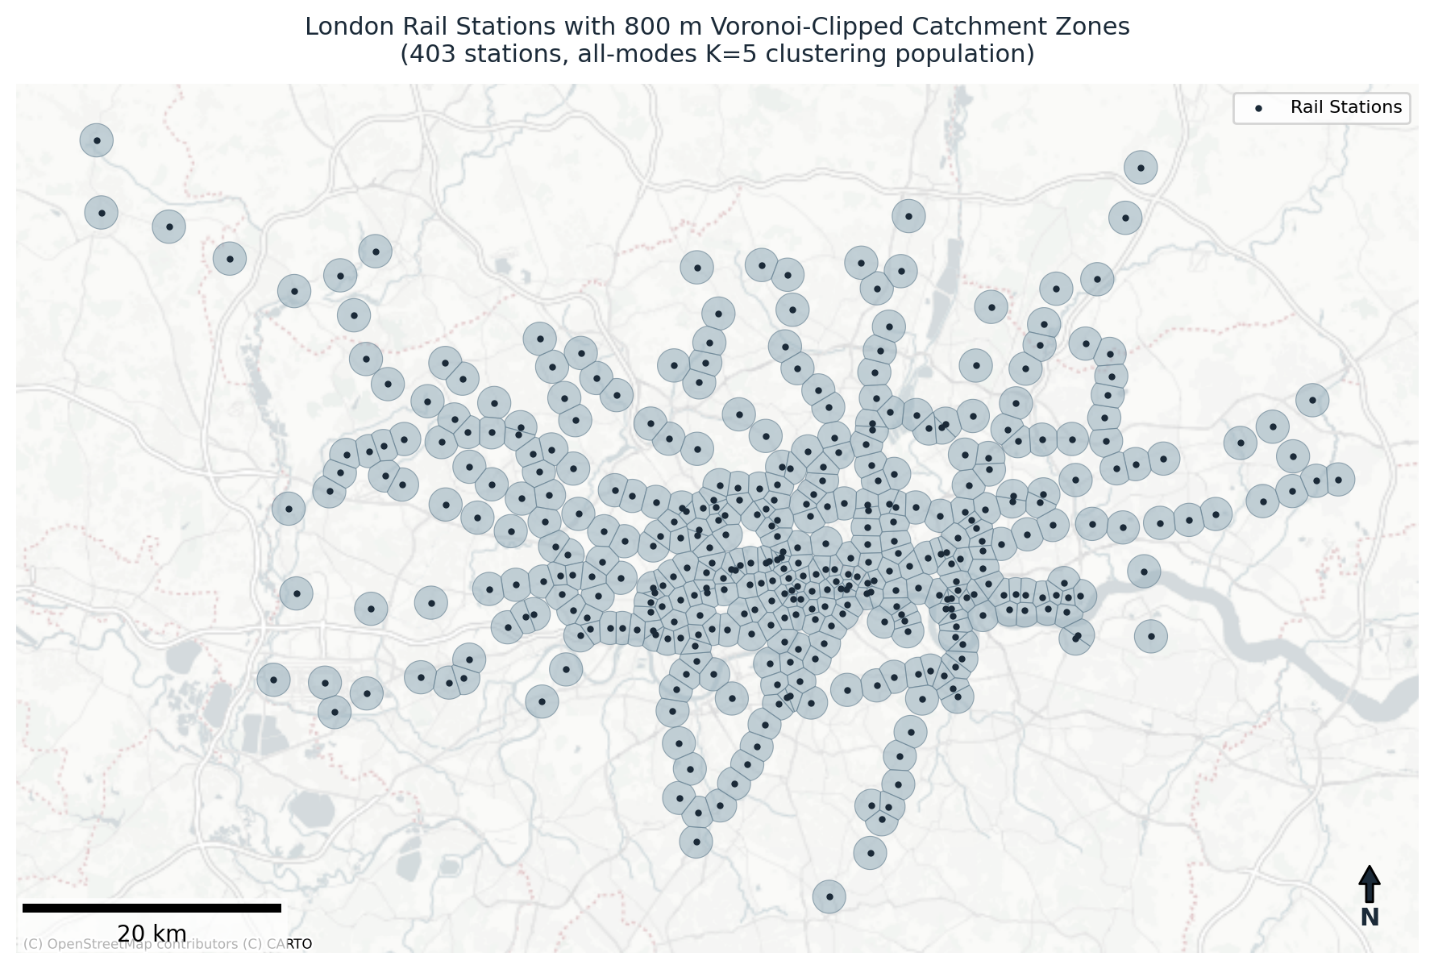
\includegraphics[width=\textwidth]{figures/v5_ch3_voronoi.png}
\caption[Rail station catchment zones]{The London rail stations with their respective hybrid Voronoi-clipped catchment zones}
\end{figure}

Each catchment was intersected with the 2021 LSOA boundaries, and duplicate geometry fragments were collapsed to make sure each distinct station--LSOA pair was represented once.

Of the 403 Rail stations included in the clustering, 389 had at least one eligible 2021 London LSOA intersecting their 800-metre Voronoi-clipped catchment and were retained for the contextual analyses. The remaining 14 stations were outer-network locations whose catchments did not intersect the spatial extent of the available London LSOA contextual data; they were excluded from the contextual analyses only and remained part of the clustering.

Station context was defined as the distribution of LSOA-level conditions among the distinct LSOAs intersecting the 800-metre Voronoi-clipped catchment. Each intersecting LSOA received equal weight, irrespective of its population or the proportion of its area falling within the catchment.

For continuous social indicators, station-level values were calculated as the arithmetic mean of the intersecting LSOAs. LNWC was summarised as a seven-part composition, representing the proportion of intersecting LSOAs in each class. The same catchments and equal LSOA weighting were used in both cases.

\subsubsection{Correspondence with the Geography of Night Work}

The first contextual analysis assessed whether the fixed transport-use clusters align with the independently derived LNWC geography. Because Bus and Rail are defined at different spatial scales, mode-specific methods were used. Bus LSOAs each carry a single LNWC category, whereas Rail station catchments are represented as seven-part LNWC compositions because individual rail catchments often intersect multiple LSOAs with different LNWC types.

For Bus, both cluster membership and LNWC type are categorical variables at LSOA level. Their association was tested using Pearson's chi-square test of independence, with effect size summarised by Cramér's V \citep{Cramer1999}:

\begin{equation}
V = \sqrt{\frac{\chi^2}{n \cdot \min(r-1,\, c-1)}}
\end{equation}

where $\chi^2$ is the chi-square statistic, $n$ is the number of Bus LSOAs, and $r$ and $c$ are the numbers of rows and columns in the contingency table.

For Rail, each of the 389 stations is described by a seven-part LNWC composition based on equal weighting of intersecting classified LSOAs. Differences in these compositions across fixed Rail clusters were evaluated using a label-permutation test. Cluster labels were randomly reassigned 999 times while station-level compositions were held constant. The observed $R^2$, defined as the ratio of between-cluster to total compositional variation, was compared against this null distribution to test whether observed differences exceed those expected under random assignment \citep{Anderson2001}:

\begin{equation}
R^2 = \frac{SS_{between}}{SS_{total}}
\end{equation}

To interpret the direction of association, enrichment ratios were calculated for each cluster and LNWC type as the share of an LNWC type within a cluster divided by its share across the relevant eligible benchmark --- the 3,383 eligible fitted Bus LSOAs, or the equal-station-weighted composition across the 389 eligible Rail stations:

\begin{equation}
ER_{kg} = \frac{s_{kg}}{s_{\cdot g}}.
\end{equation}

A value above one indicates over-representation relative to that benchmark. Where a cluster showed one clearly strongest enrichment, that LNWC type was used as a concise contextual label.

\subsubsection{Differences in Urban Background Indicators Across Clusters}

The 20 continuous urban background indicators were analysed after clustering, using fixed cluster labels as grouping variables. These indicators were not used in cluster construction or refinement. The analysis instead examined whether contextual distributions differed across transport-use types. Rail and Bus were analysed separately, using 389 Rail station catchments and 3,383 Bus LSOAs.

For each indicator, a Kruskal--Wallis test assessed whether distributions differed across clusters within each mode \citep{Kruskal1952}. This non-parametric test was used because the variables included bounded proportions and skewed counts that did not meet ANOVA assumptions. Benjamini--Hochberg correction was applied across the 20 tests separately for Rail and Bus \citep{Benjamini1995}.

$\varepsilon^2$ was used to rank the magnitude of between-cluster differentiation across the 20 indicators within each mode:

\begin{equation}
\varepsilon^2 = \frac{H - k + 1}{n - k},
\end{equation}

where $H$ is the Kruskal-Wallis statistic, $k$ is the number of clusters and $n$ is the number of units in the test.

To identify which clusters drove these differences, each cluster was compared with all remaining units using two-sided Mann--Whitney U tests. Rank-biserial correlation was used to describe direction and magnitude. Benjamini--Hochberg correction was applied across 80 Bus comparisons (4 clusters $\times$ 20 indicators) and 100 Rail comparisons (5 clusters $\times$ 20 indicators).

Standardised cluster-mean z-scores were reported as descriptive summaries, indicating whether each cluster was above or below the mode-wide mean. Inference was based on the Kruskal--Wallis and Mann--Whitney results, their effect sizes, and adjusted p-values.

\section{Ethical Considerations and Methodological Boundaries}

This study used publicly available, aggregate transport and area-level contextual data. No personal identifiers, individual smart-card records or individual movement trajectories were accessed, and the research involved no participant recruitment or direct interaction with human subjects.

Socio-economic and demographic indicators were interpreted only as characteristics of the surrounding areas. They were not treated as attributes of individual passengers, and the analysis does not infer individual travel behaviour from area-level associations.

Generative AI tools were used in an assistive capacity for code development, debugging and language proofreading. All analytical decisions, interpretation and final written content remain the responsibility of the author.
